\begin{figure}
  \centering
  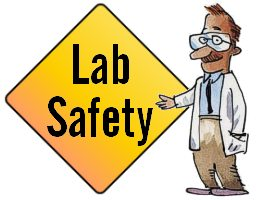
\includegraphics[width=0.3\textwidth]{fig/labsafety.jpg}
\end{figure}

\section*{Safety Instructions and General Guide for the Physical Chemistry Laboratory Practice}
\addcontentsline{toc}{section}{Appendix A -- Safety instructions}


Working in a chemistry laboratory can be dangerous. You are exposed to a wide range of chemicals, flame, high temperature devices ie. hotplate, high pressure containers, sharp tools, fragile glassware. Safe laboratory practice is essential to prevent any injury to yourself, and others.

First and foremost, you should always be prepared for your current laboratory practice. You should be familiar with the topic. Prepare for the practice in advance. Depending on the subject spend at least 2 hours with preparations by studying the handout carefully in the day before the pactice, and about 15 minutes before the practice. Understand the task at hand. If you don't know what you are doing, you will make mistakes, unnecessarily prolong the practice, endanger yourself and others, and ultimately fail. With good preparation however, the practice will be useful, successful, and even fun.

\begin{enumerate}
\item You may carry to the laboratory only the following items:
	\begin{itemize}
	\item your notebook,
	\item pen,
	\item marker,
	\item calculator,
	\item labcoat,
	\item your own spatula if you have one.
	\end{itemize}
\item You may NOT carry these to the laboratory:
	\begin{itemize}
	\item food,
	\item drinks,
	\item your bag,
	\item jacket,
	\item umbrella.
	\end{itemize}
\item You may NOT do these in the laboratory:
	\begin{itemize}
	\item eat,
	\item drink,
	\item smoke,
	\item do any other practice than your own,
	\item be alone in the laboratory.
	\end{itemize}
\end{enumerate}

Always wait for the supervising teacher to arrive before you enter the laboratory. Be punctual, arrive at least 5 minutes before the practice starts, at the entrance, ready for the work. Leave your bag, jacket, umbrella etc. in your locker at the designated area. Do not leave anything at the entrance.
	
Start your work by cleaning your work area. Then wash everything (eg. glassware, electrodes, cuvettes, beakers, flasks, spatulas, pipettes, burettes) first by tapwater. Use detergents and scrubber if necessary. Then, flush them with ionized water, or double deionized water, depending on the requirements of the practice. For example to determine the solubility product of a sparingly soluble salt, both the electrodes, and the glassware have to be extremely clean. Wash glassware with great care for these practices. The quality of your work will depend on your effectiveness of cleaning.

It is VERY important to write down everything you do in the laboratory. A short guide about this can be found in the foreword of your practice handouts. Precise record keeping is essential for the evaluation of your work. Write down your observations, measured data, the precise time if possible, and even the results of unsuccessful work. These might turn out to be "successful" experiments later.

Always label every solution you prepare with a marker. If you are unsure about the content of an unlabeled container, don't use it! Use only labeled chemicals. It is strongly advised to bring your own marker to the practice instead of constantly keep borrowing someone else's.

Never use broken equipment. If you notice a crack or even the smallest one, dispose it in the designated waste container. Always notify the laboratory supervisor about broken equipment.

Dispose aqeous solutions with low environmental hazard into the sink. Use excess water to wash it down. Carefully neutralize concentrated acids and bases before disposing. There is an organic solvent waste located below the fume hood. You may dispose organic waste into this container only. Do not throw solids in the sink eg. pieces of broken glass, spatulas, paper towels. Do not pour fluids into the sink if there is a magnetic stirrer in it. Remove the stirrer first.

Use protective equipment if necessary. Latex gloves and safety glasses will be in your drawer. Always wear your labcoat during the entire practice. It is advised to button your coat. Do not wear open shoes. Tie your hair up if it's long.

Do not smell chemicals directly. Use your hands as a fan instead to smell the chemical. Do not taste any chemical under any circumstances! If a chemical is accidentally swallowed, wash it with excessive water, and notify the supervisor immediately!

We won't use open flame during this practice. If there is a fire however, you can find fire extinguishers in the lab, and in the corridor. There is an emergency shower located above the door in the laboratory. Use this immediately if your cloth catches on fire. Stand below the shower, and pull the lever. The elevators may not be used during a fire alarm. In case of a fire alarm, use the emergency stairs to exit the building.

Fire will persist of there is flammable material, enough oxygen, and high enough temperature. Remove any of these, and the fire will stop. The building has an automatic ventillation system. The windows cannot be opened. You can cover the fire with a blanket or a piece of wet clothing to prevet oxygen resupply to the fire. Depending on the fire, use different fire extinguishers. To extinguish electric fire, do not use water based extinguishers! Use only dry chemical extinguiser in these cases.

There is a first aid kit in the laboratory to provide basic medical assistance. If acids or bases are spilled on your skin, use plenty of water to wash it, then use 2\% sodium-hydroge-carbonate and 2\% acetic acid for injuries caused by acids and bases, respectively. If these are spilled into your eyes, use 2\% sodium-borate (borax), and 2\% boric-acid for acids and bases, respectively, after washing it with plenty of water. 

In case of gas intoxication, get fresh air immediately. As the windows are not openable in our laboratory, you should get out of the building immediately accompanied by at least two other people. Notify the supervisor in any case of intoxication or injury! Use fume hood for the practices using volatile chemicals (chloroform, cc. acetic-acid). If acid is swallowed, DO NOT swallow sodium-carbonate to neutralize it, as a huge amount of carbon-dioxide could potentially evolve, and the injured stomach might rupture. In case of electrical shock, notify the supervisor, and seek medical assistance immediately!


\begin{figure}
  \centering
  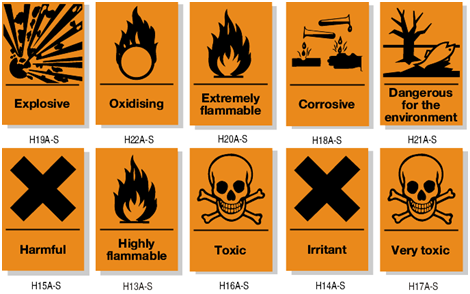
\includegraphics[width=1\textwidth]{fig/old_hazard.png}
  \caption{Old chemical hazard symbols.}
\end{figure}


\begin{figure}
  \centering
  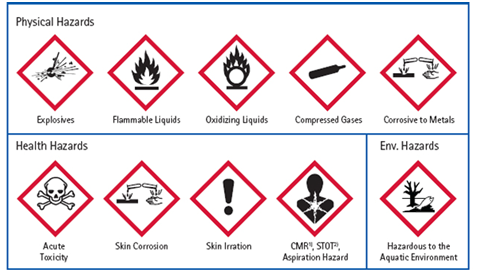
\includegraphics[width=1\textwidth]{fig/new_hazard.png}
  \caption{New chemical hazard symbols.}
\end{figure}
